\title{Лекция 19\\Представление в базе знаний задач и их решений}
\author[]{Шункевич Д.В.}
\institute[]{Белорусский государственный университет информатики и радиоэлектроники}

\begin{frame}
	\titlepage
\end{frame}

\begin{frame}{\\Содержание лекции}
	\topline
	\justifying
	Понятие задачи, классификация задач. Информационные и поведенческие задачи. Декларативная и процедурная формулировка задачи. Понятие плана выполнения действия, протокола выполнения действия, результата выполнения действия. Примеры описания решения задачи в базе знаний. Понятие команды. Принципы работы с командами в интерфейсе компьютерных систем нового поколения. 
\end{frame}

\begin{frame}{\\Понятие задачи}
	\topline
	\justifying
    \begin{SCn}
    \scnheader{задача}
    \scnidtf{описание некоторого желаемого состояния или события либо в базе знаний, либо во внешней среде}
    \scnidtf{формулировка задачи}
    \scnidtf{задание на выполнение некоторого действия}
    \scnidtf{постановка задачи}
    \scnidtf{задачная ситуация}
    \scnidtf{спецификация некоторого действия, обладающая достаточной полнотой для выполнения этого действия}
    \end{SCn}
\end{frame}

\begin{frame}{\\Понятие задачи}
	\topline
	\justifying
    \textbf{\textit{Задача}} задаётся отношением  между описанием исходной ситуации и описанием целевых ситуаций.\\
    
    \bigskip
    
    Каждая \textbf{\textit{задача}} представляет собой спецификацию действия, которое либо уже выполнено, либо выполняется в текущий момент (в настоящее время), либо планируется (должно) быть выполненным, либо может быть выполнено (но не обязательно). 
\end{frame}

\begin{frame}{\\Классификация задач}
	\topline
	\justifying
 
    Классификация задач может осуществляться по дидактическому (логическому) признаку в рамках каждой предметной области (задачи на треугольники, задачи на системы уравнений и т.п.)\\
    \bigskip
    Каждая \textit{задача} может включать:
    \begin{textitemize}
        \item факт принадлежности \textit{действия} частному классу \textit{действий}, в том числе состояние \textit{действия} с точки зрения жизненного цикла (инициированное, выполняемое и т.д.);
        \item описание \textit{цели*} (\textit{результата*}) \textit{действия}, если она точно известна;
        \item указание \textit{заказчика*} действия;
        \item указание \textit{исполнителя* действия};
    \end{textitemize}
\end{frame}

\begin{frame}{\\Классификация задач}
	\topline
	\justifying
    
    \bigskip
    Каждая \textit{задача} может включать:
    \begin{textitemize}
        \item указание \textit{аргумента(-ов) действия\scnrolesign};
        \item указание инструмента или посредника \textit{действия};
        \item описание \textit{декомпозиции действия*};
        \item указание \textit{последовательности действий*} в рамках \textit{декомпозиции действия*}, т.е. построение процедурного плана решения задачи;
        \item указание области \textit{действия};
        \item указание условия инициирования \textit{действия};
        \item момент начала и завершения \textit{действия}, в том числе планируемый и фактический, предполагаемая и/или фактическая длительность выполнения.
    \end{textitemize}
\end{frame}

\begin{frame}{\\Классификация задач}
    \topline
	\justifying
 
    \bigskip
    
    Некоторые задачи могут быть дополнительно уточнены контекстом -- дополнительной информацией о сущностях, рассматриваемых в формулировке \textit{задачи}, т.е. описанием того, что дано, что известно об указанных сущностях.\\
    \bigskip
    
    Кроме этого, \textit{задача} может включать любую дополнительную информацию о действии, например:
    \begin{textitemize}
        \item перечень ресурсов и средств, которые предполагается использовать при решении задачи;
        \item ограничение области, в которой выполняется \textit{действие};
        \item ограничение знаний, которые можно использовать для решения той или иной задачи.
    \end{textitemize}
\end{frame}

\begin{frame}{\\Информационные и поведенческие задачи}
	\topline
	\justifying

    Как и в случае с действиями, решаемыми системой, можно классифицировать \textit{информационные задачи} и \textit{поведенческие задачи}. 
    С другой стороны, с точки зрения формулировки поставленной задачи, можно выделить \textit{декларативные формулировки задачи} и \textit{процедурные формулировки задачи}. Следует отметить, что данные классы задач не противопоставляются друг другу, и могут существовать формулировки задач, использующие оба подхода.
\end{frame}

\begin{frame}{Декларативная и процедурная формулировка задачи}
	\topline
	\justifying
     
    \begin{SCn}
    \scnheader{задача}
    \scnsuperset{вопрос}
    \scnsuperset{команда}
    \scnsubset{знание}
    \scnsuperset{инициированная задача}
    \scnsuperset{декларативная формулировка задачи}
    \scnsuperset{процедурная формулировка задачи}
    \scnsuperset{декларативно-процедурная формулировка задачи}
    \scnsuperset{задача, решаемая в памяти кибернетической системы}
    \end{SCn}
\end{frame}

\begin{frame}{Декларативная и процедурная\\ формулировка задачи}
	\topline
	\justifying
  
    \textbf{\textit{декларативная формулировка задачи}} представляет собой описание начальной ситуации, являющейся условием выполнения соответствующего действия, и целевой ситуации, являющейся результатом выполнения этого действия, то есть  описание состояния, которое должно быть достигнуто в результате выполнения планируемого действия. 
\end{frame}

\begin{frame}{Декларативная и процедурная\\ формулировка задачи}
	\topline
	\justifying
     В случае \textbf{\textit{процедурной формулировки задачи}} явно указывается характеристика действия, специфицируемого этой задачей, а именно, например, указывается:
    \begin{textitemize}
    \item субъект или субъекты, выполняющие это действие;
    \item объекты, над которыми действие выполняется, -- аргументы действия;
    \item инструменты, с помощью которых выполняется действие;
    \item момент и, возможно, дополнительные условия начала и завершения выполнения действия;
    \item класс или классы, которым принадлежит каждое \textit{действие}.
    \end{textitemize}	
    
	При этом явно не уточняется, что должно быть результатом выполнения соответствующего действия. 
    
\end{frame}

\begin{frame}{Декларативная и процедурная\\ формулировка задачи}
	\topline
	\justifying
	\vspace{10mm}
	
    Заметим, что, при необходимости, \textit{процедурная формулировка задачи} может быть сведена к \textit{декларативной формулировке задачи} путем трансляции на основе некоторого правила, например, определения класса действия через более общий класс.
    
    \bigskip
    
    Декларативно-процедурная формулировка задачи -- задача, в формулировке которой присутствуют как декларативные (целевые), так и процедурные аспекты.  Инициированная задача -- формулировка задачи, которая подлежит выполнению.
    
\end{frame}

\begin{frame}{\\Частные виды задач}
    \topline
	\justifying
    \begin{SCn}
    \scnheader{вопрос}
    \scnsubset{задача, решаемая в памяти кибернетической системы}
    \scnidtf{непроцедурная формулировка задачи на поиск (в текущем состоянии базы знаний) или на генерацию знания, удовлетворяющего заданным требованиям}
    \scnidtf{задача, направленная на удовлетворение информационной потребности некоторого субъекта-заказчика}
    \scnheader{команда}
    \scnidtf{инициированная задача}
    \scnidtf{спецификация инициированного действия}
    \end{SCn}
\end{frame}

\begin{frame}{\\Понятие плана выполнения действия}
	\topline
	\justifying
    \scnheader{план выполнения действия}
    \scnidtf{процедурная программа}
    \scnidtf{спецификация декомпозиции любого действия, принадлежащего заданному классу действий}
\end{frame}

\begin{frame}{\\Понятие протокола выполнения действия}
	\topline
	\justifying
    \scnheader{протокол выполнения действия}
    \scnidtf{описание того, как действительно было выполнено соответствующее действие и, в частности, описание последовательности соответствующих ситуаций и событий}
    \scnidtf{декомпозиция выполненного действия на систему последовательно-параллельно выполненных его
поддействий}
 
\end{frame}

\begin{frame}{\\Понятие результата выполнения действия}
	\topline
	\justifying
 
    \bigskip
    
    Результат -- отношение, которое  связывают sc-элемент, обозначающий действие, и sc-конструкцию, описывающую результат выполнения рассматриваемого действия, другими словами, цель, которая должна быть достигнута при выполнении действия.\\
    Результат может специфицироваться как атомарным высказыванием, так и неатомарным, т.е. конъюнктивным, дизъюнктивным, строго дизъюнктивным и т.д.\\
    
    \bigskip
    
    В случае, когда успешное выполнение действия приводит к изменению какой-либо конструкции в sc-памяти,  которое необходимо занести в историю изменений базы знаний или использовать для демонстрации протокола решении задачи, генерируется соответствующая связка отношения результат*, связывающая  задачу и sc-конструкцию, описывающую данное изменение. 
\end{frame}

\begin{frame}{\\Понятие команды}
	\topline
	\justifying
	\vspace{10mm}

    \scnheader{команда}
    \scnidtf{инициированная задача}
    \scnidtf{спецификация инициированного действия}
    
   \bigskip
    
   Идентификатор экземпляров конкретного класса команд в рамках Русского языка пишется с прописной буквы и представляет собой либо содержащее глагол совершенного вида в инфинитиве описание сути того, что требуется получить в результате выполнения действия, соответствующего данной команде, либо вопросительное предложение, являющееся спецификацией запрашиваемой (ответной) информации.
   
   \bigskip
   
   Например:
   \begin{textitemize}
   		\item "Что такое треугольник?"
   		\item "Сгенерировать новый экземпляр класса треугольник"
   \end{textitemize}
   
\end{frame}

\begin{frame}{\\Пример условия задачи}
	\topline
	\justifying
	\vspace{10mm}
	\begin{SCn}
		\begin{figure}[H]
			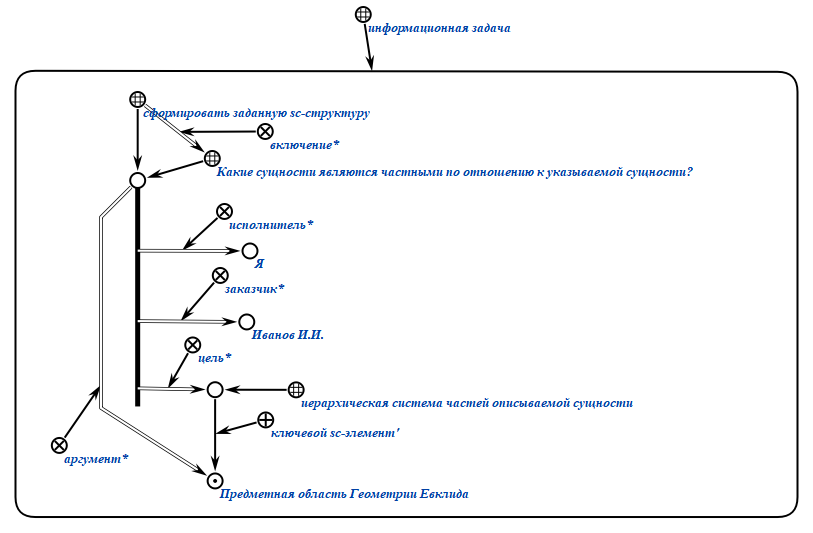
\includegraphics[scale=0.5]{./figures/sd_problems/entities.png}
		\end{figure}
	\end{SCn}
\end{frame}

\begin{frame}{\\Пример условия задачи}
	\topline
	\justifying
	\vspace{10mm}
	\begin{SCn}
		\begin{figure}[H]
			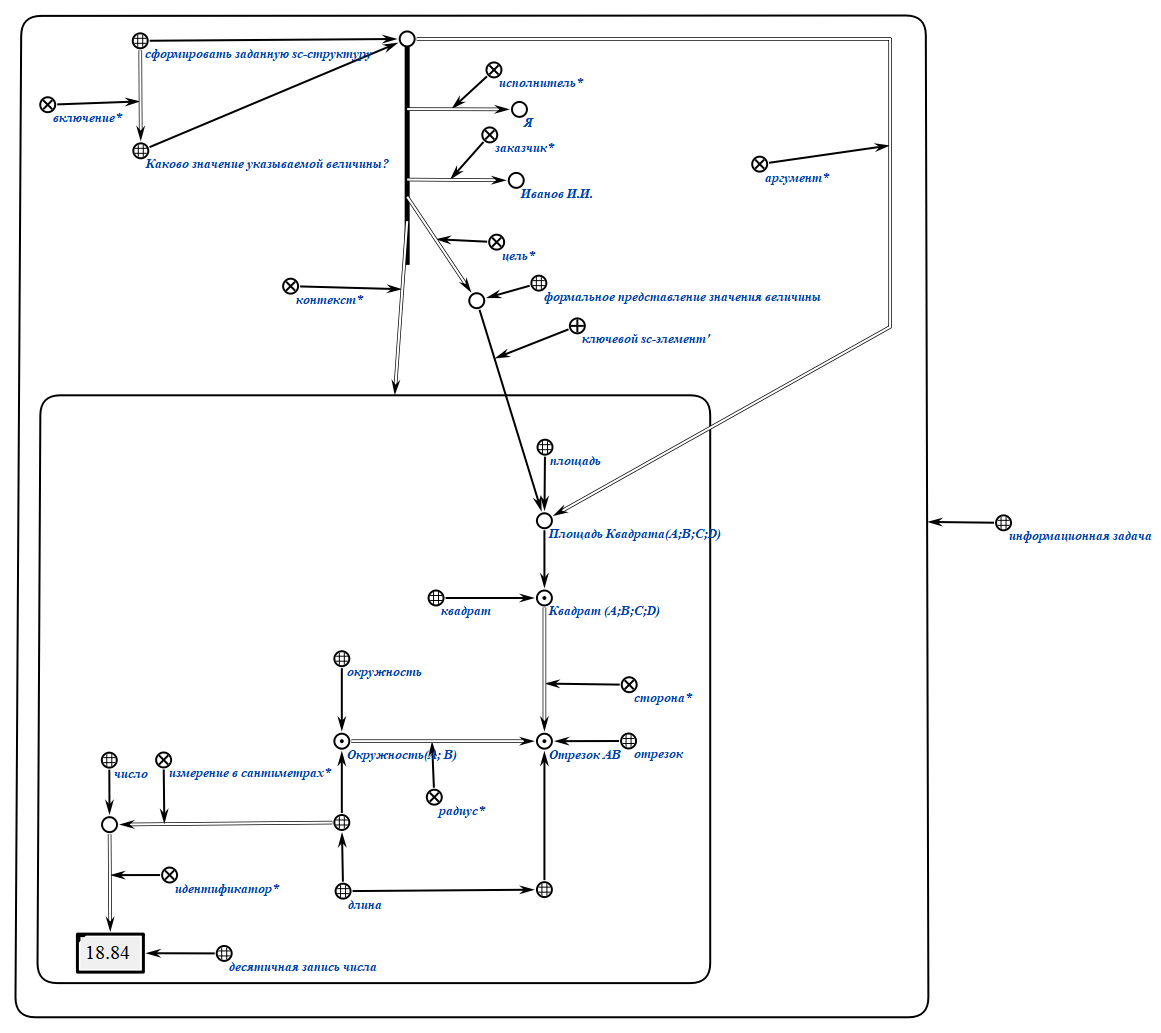
\includegraphics[scale=0.3]{./figures/sd_problems/value.png}
		\end{figure}
	\end{SCn}
\end{frame}


\begin{frame}{\\Пример решения задачи}
	\topline
	\justifying
	\vspace{10mm}
	\begin{SCn}
		\begin{figure}[H]
			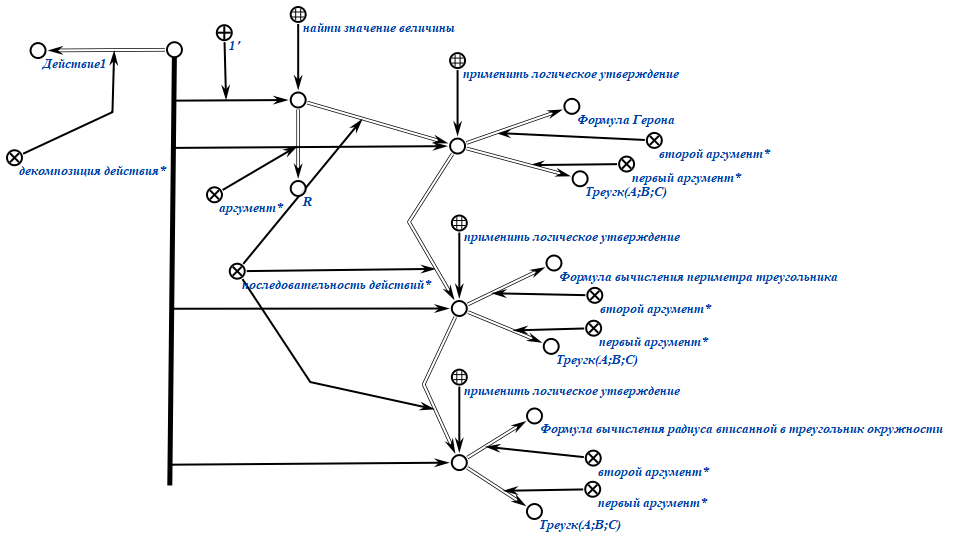
\includegraphics[scale=0.47]{./figures/sd_problems/solution.png}
		\end{figure}
	\end{SCn}
\end{frame}